\documentclass{source/Paper}

\name{name}
\articletitle{PSI from Ring-OLE: Review}
\stuid{stuid}
\date{\today}
\course{Data Security and Privacy Protection}

\Abstract{PSI from Ring-OLE is the latest PSI protocol, and it outperforms previous work in certain scenarios. We first introduce the contribution and background of this paper, then we outline building blocks. We followed by analyzing the advantages and disadvantages of the protocol, and finally  summarize the paper.}


\Keyword{PSI; OLE; Ring-OLE}

\begin{document}

    \makeheader
    \section{Introduction}
    This paper\cite{chongchitmate2022psi} was proposed by Chongchitmate et al. in 2022 and discussed Private Set Intersection and its variants, including PSI-Payload and PSI+Sum. PSI is a cryptographic protocol that allows two parties to find the intersection of their sets without revealing any additional information. In other words, one of the parties cannot obtain any information about the elements of the non-intersecting part of the other party. PSI+Sum is an extension of PSI, where, instead of learning the intersection, the receiver learns the sum of the associated payloads. PSI-Sum is the standard protocol that does not compute the intersection of two set, but only the sum of the associated payloads of the intersection. So PSI+Sum is a relaxed version of PSI-Sum.

    This paper makes two related contributions. First, they construct simple and efficient protocols for PSI and PSI-Payload from a ring version of oblivious linear function evaluation (Ring-OLE). And the second contribution is an efficient general reduction of a variant of PSI-Sum to PSI-Payload and secure inner product.

    This paper also mentioned techniques used in other PSI protocols that and how they can be used in constructing PSI protocols. They compared different PSI protocols and discussed their communication complexity and running time under different setting. Compared to previous maliciously secure PSI protocols that have a similar computational cost, online communication of this paper is 2x better for small sets ($2^8$ - $2^{12}$ elements) and 20\% better for large sets ($2^{20}$ - $2^{24}$ elements).
    \section{Techniques}
    \textbf{OLE:} 

    OLE is short for oblivious linear function evaluation.
    Let $\mathbb{F}$  be a finite field. An oblivious linear function evaluation allows two parties, a sender with input $a,b \in \mathbb{F} $ and a receiver with input $x \in \mathbb{F} $, to securely compute $ax + b$ and output to the receiver.
    The OLE can be seen as a generalization of an oblivious transfer
    (OT) where $\mathbb{F} = \mathbb{F}_2 $.

    \textbf{Ring-OLE:}

    Ring-OLE is OLE for polynomial ring.
    This is used for constructing simple and efficient protocols for PSI and PSI-Payload. Ring-OLE generalizes OLE to a ring, particularly a polynomial ring. We can use OLE to construct Ring-OLE. Let $c$ be an element of a finite field and $a,b,x$ be elements of a polynomial ring.
    The receiver holds $x$ and the sender holds $a,b$. So the receiver computes $x(c)$ and the sender computes $a(c),b(c)$, then they use the OLE protocol and the receiver will get $a(c)x(c)+b(c)$. Using Lagrange polynomial interpolation, the receiver will get the polynomial which equals $ax+b$.

    \textbf{Secure inner product:}

    A secure inner product functionality allows two parties to compute an inner product of each party's input vector and output as an additive share to each party. Specifically, the sender holds $\vec{v}$ and $\vec{r}$ and the receiver holds $\vec{u}$. Using OLE, the receiver will get $\vec{v}\cdot \vec{u} - \sum r$ and the sender knows the other share $ \sum r$.



    \section{Strengths}

    This paper solved the PSI problem using an algebraic approach which is efficient and secure. We use a polynomial to represent a set whose roots are the elements in the set. This means that, given a set $A=\{ a_1,a_2,\cdots,a_n\}$, we can construct a polynomial $f(x)=\prod_{i=1}^{n}(x-a_i)$ to represent the set $A$. Polynomial representation is common in previous work, but most of the previous work used encryption to securely transfer polynomials, such as homomorphic encryption, and then compute the addition and multiplication of polynomials. This paper used Ring-OLE to compute the output polynomial and there is a large improvement in communication cost and computation cost. First, homomorphic encryption uses public key cryptography, and the length of ciphertext will be large in most cases. Secondly, both addition and multiplication operations of homomorphic encryption will be much slower than addition and multiplication of plaintext.

    This protocol significantly increases efficiency in the online phase by moving all calls to the Ring-OLE functionality to the offline phase. The online phase is non-cryptographic and typically has higher efficiency in both communication and running time compared to other PSI protocols, even those with only semi-honest security. The pre-processing phase included operations independent of the set size and the set elements, so we can perform calculations in advance, saving a lot of time. As is shown in Figure \ref{f1}, compared to the state-of-the-art OT-based PSI with semi-honest security, the communication complexity of our PSI protocol in the online phase is up to 50\% smaller while remaining competitive in the running time for small($2^{8},2^{12}$ elements) sets. The vector-OLE-based PSI and DH-based PSI only outperform ours in term of communication for large ($2^{20},2^{24}$ elements) sets.


    \begin{figure}[H]
        \centering
        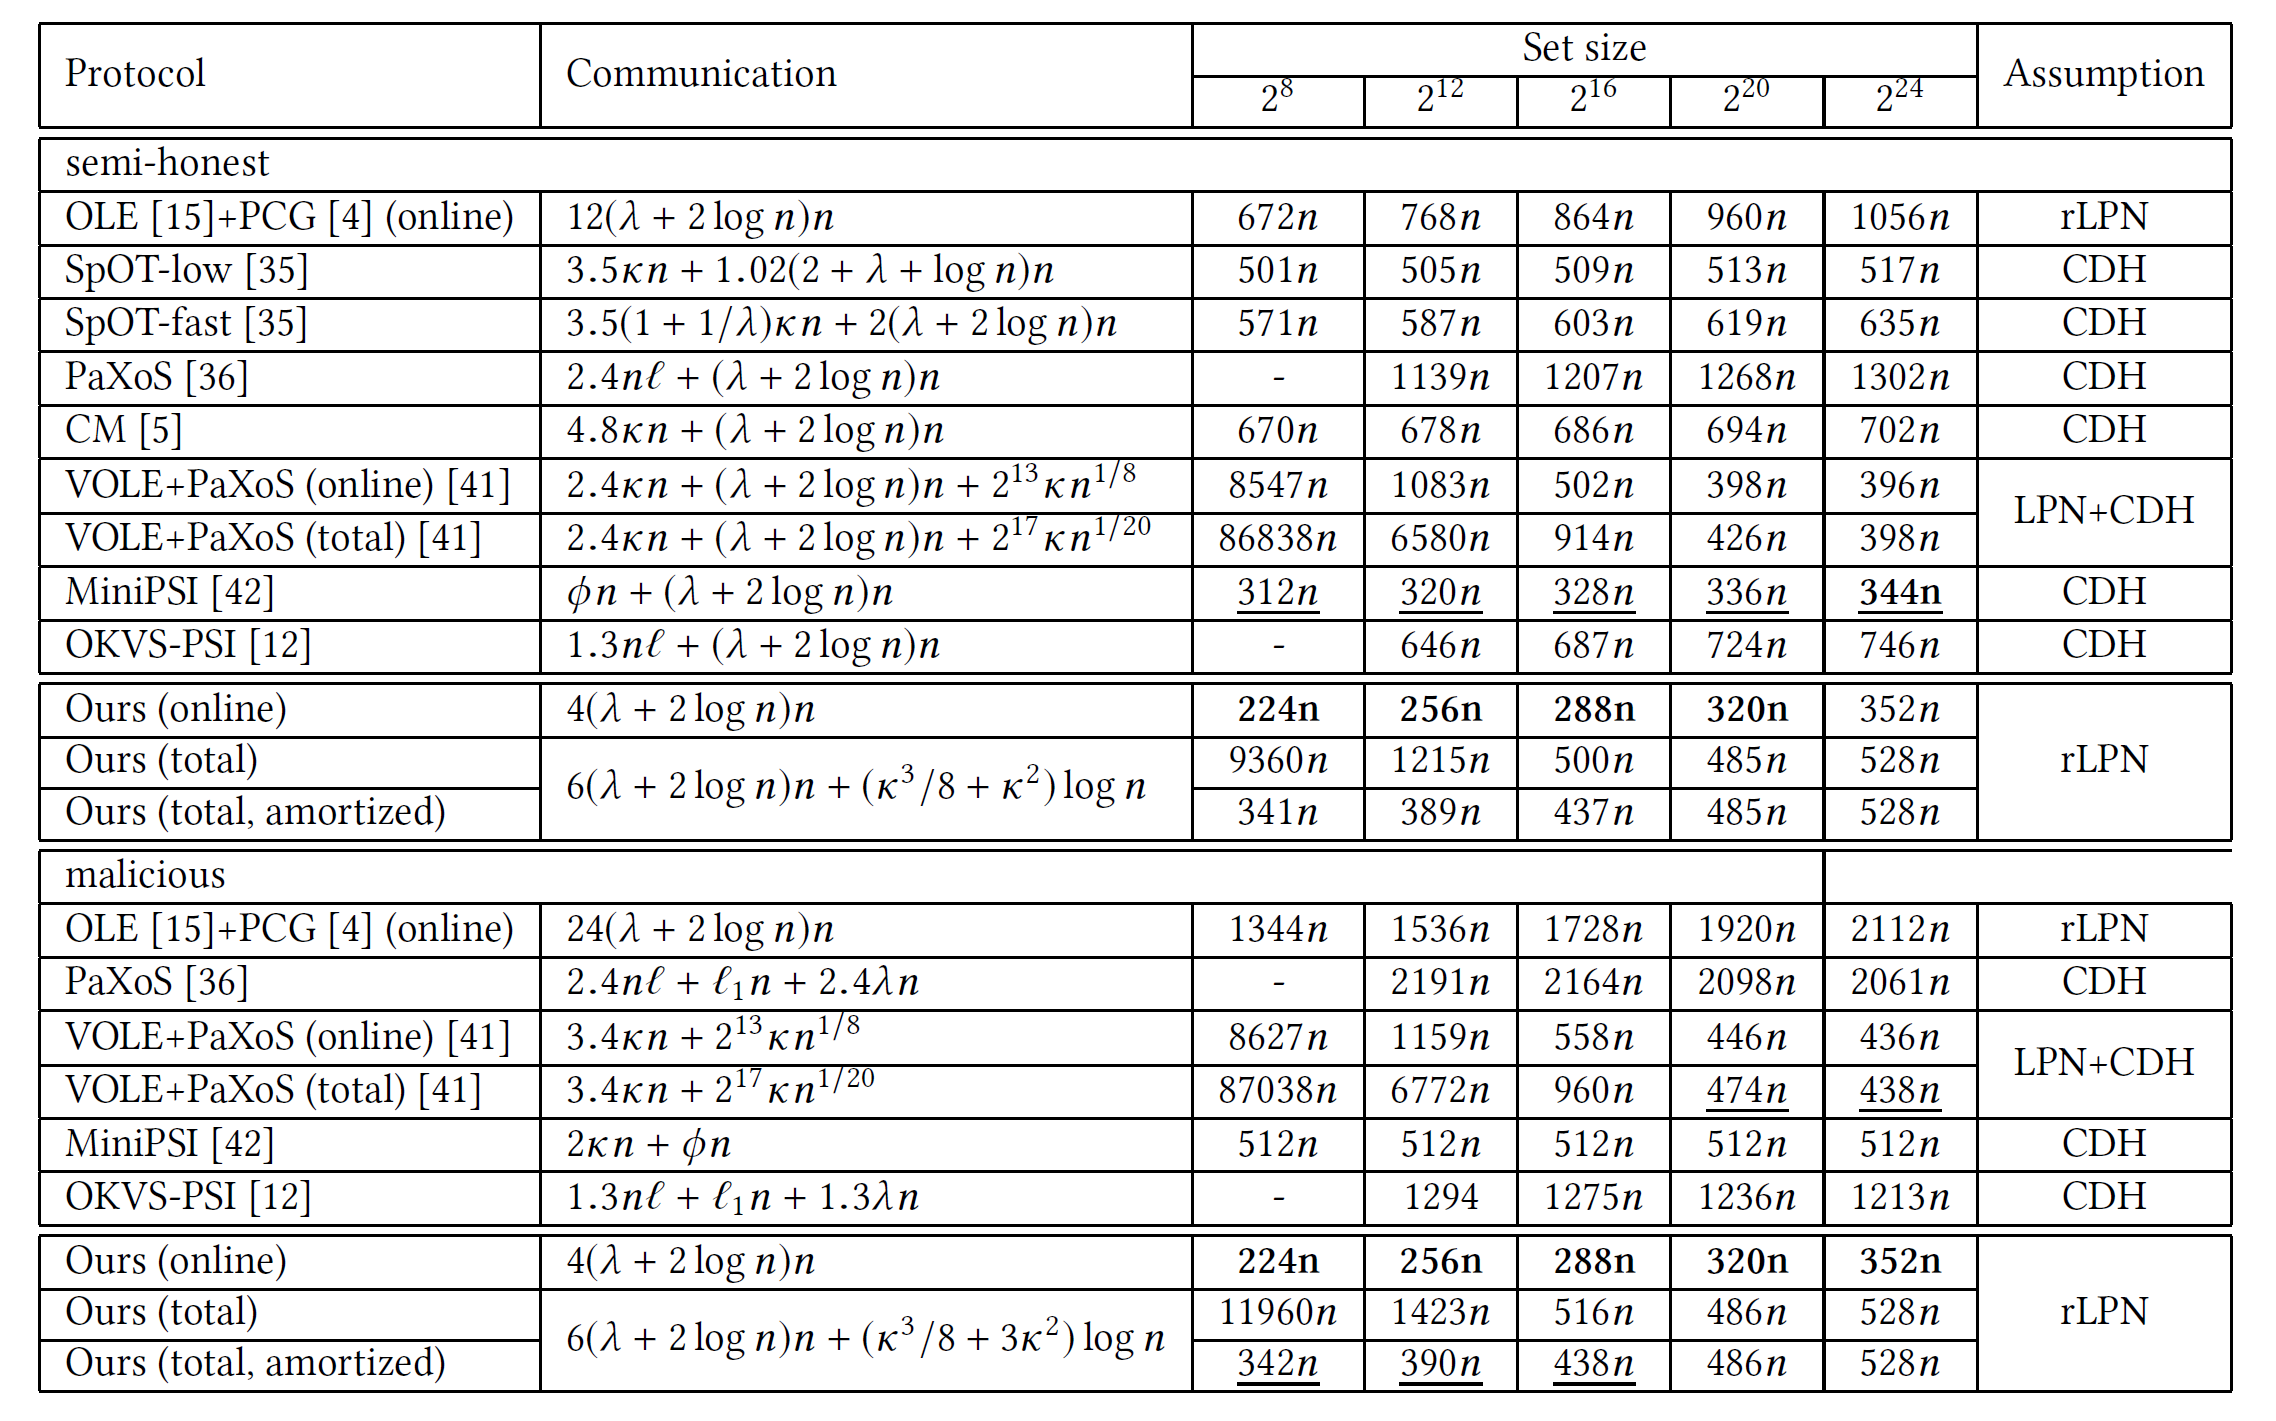
\includegraphics[width=0.8\linewidth]{pic/perform.png}
        \caption{\textbf{Communication of PSI protocols}}
        \label{f1}
    \end{figure}

    The algebraic-based approach can be easily extended from semi-honest models to malicious models. This paper also benefits from this. The overhead of this protocol is the same under the semi-honest model and the malicious model, a feature that is rarely found in other PSI protocols. There is no doubt that the protocol is very efficient under the malicious model compared to other methods. At the same time, the algebraic approach easily implements the PSI-Payload and PSI+Sum. Unfortunately, the protocol does not achieve the standard PSI-Sum.

    \section{Weaknesses}

    This paper still has some weaknesses. First, the protocol is not suitable for unbalanced scenarios, where there is a large gap between the set sizes of receiver and sender. 
    This paper used padding to ensure that the sets of both sides reach the same size, which is certainly not appropriate for unbalanced scenarios. To protect privacy, the degree of the output polynomial is determined by the larger of the two sets. For example, the receiver is a computationally weak device, a cell phone, etc. The receiver's data size is relatively small, but it needs to receive a large output polynomial and evaluate the polynomial. This is a huge overhead for both computation and communication. 

    The protocol has relatively high security parameters which is $4(\lambda + 2\, \mathrm{log}\, n)$. Intuitively, the communication overhead of the protocol should be linearly related to the set size. However, due to the polynomial representation, the size of the domain is important. The protocol needs to choose a domain large enough to avoid collisions of polynomial roots. 
    Therefore the protocol has a super-linear communication overhead. 

    Despite the use of the FFT algorithm, Lagrange polynomial interpolation is still the most time-consuming of the whole protocol. Polynomial valuation is also time consuming and the recipient is responsible for the overhead. 

    \section{Summary and Comment }
    Ring-OLE is a very useful cryptographic primitive which avoids the use of encryption to efficiently compute polynomials. Using a random polynomial to protect the original polynomial is a good idea. It is similar to adding two numbers together to hide the original number without the homomorphic encryption.

    Polynomial representation is more efficient in communication, but slower in computation. Therefore using polynomial approach can further optimize the protocol in terms of communication overhead. The existing PSI protocols are already excellent in terms of computational performance, but the communication overhead is still not satisfactory. Even if the data in the set does not have 128 bits, we still need to use an encryption scheme with a long ciphertext length to protect privacy. For example, given a set of integers under $2^{32}$, we still have to use a 128-bit secure encryption scheme. On the other hand, the network in most scenarios will not be LAN and the time to transfer data is non-negligible.

    The algebraic approach not only plays a great role in PSI protocols, but can also be used in PSU protocols which aim to compute the union of two sets. In the future, communication overhead will be one of the research hotspots for both PSI and PSU protocols, since most of the data is scattered in individual IoT devices.


    \newpage
    \bibliographystyle{unsrt}
    \bibliography{ref}

\end{document}


